\documentclass[a4paper]{article}
\usepackage[utf8]{inputenc}
\usepackage[T1]{fontenc}
\usepackage[slovene]{babel}
\usepackage{lmodern} 
\usepackage{hyperref}
\usepackage{blindtext}
\usepackage{amsmath}  % razna okolja za poravnane enačbe ipd.
\usepackage{amsthm}   % definicije okolij za izreke, definicije, ...
\usepackage{amssymb}  % dodatni matematični simboli
\usepackage{listings} % okolje za Python kodo
\usepackage{xcolor}   % okolje za barve (za kodo)

\definecolor{codegreen}{rgb}{0,0.6,0}
\definecolor{codegray}{rgb}{0.5,0.5,0.5}
\definecolor{codepurple}{rgb}{0.58,0,0.82}

\lstdefinestyle{mystyle}{   
    commentstyle=\color{codegreen},
    keywordstyle=\color{magenta},
    numberstyle=\tiny\color{codegray},
    stringstyle=\color{codepurple},
    basicstyle=\ttfamily\footnotesize,
    breakatwhitespace=false,         
    breaklines=true,                 
    captionpos=b,                    
    keepspaces=true,                 
    numbers=left,                    
    numbersep=5pt,                  
    showspaces=false,                
    showstringspaces=false,
    showtabs=false,                  
    tabsize=2
}
\lstset{language=Python, style=mystyle}

\title{\textit{Grid-peeling}}
\author{Gašper Pust, Mitja Mandić}
\begin{document}

\begin{titlepage}
 \maketitle
\end{titlepage}

\section{Predstavitev problema}
V projektu si bova podrobneje ogledala konveksne ovojnice $m \times n$ mreže. Konveksna ovojnica množice je najmanjša konveksna množica, ki vsebuje dano množico točk.
Najlažje si jo predstavljamo tako, kot da bi okoli elementov množice napeli elastiko - kar elastika obkroži, je konveksna ovojnica. Lupljenje konveksnih ovojnic mreže,
(angl. \textit{grid-peeling}) je proces, ko iz mreže iterativno odstranjujemo konveksne ovojnice. S simboli lahko to zapišemo takole:
$ P_{0} = G_{m,n} = \{1,\ldots, m\} \times \{1, \ldots, n\}$. Naj bo $C_{i} = \mathcal{C}\mathcal{H}(P_{i-1}) \text{ za } i = 1, \ldots$. $V_{i}$ naj bo množica vozlišč $C_{i}$
- kot vozlišče razumemo točko, ki je na vogalu mreže (torej za katero bi zataknili elastiko). Naj bo sedaj $P_{i} = P_{i-1} \setminus V_{i}$. Začnemo torej z $n \times m$ mrežo 
in iterativno lupimo konveksne ovojnice, dokler ne odstranimo vseh točk.

V projektni nalogi bova s pomočjo simulacij opazovala v literaturi navedene številke za $n \times n$ mrežo - teorija napoveduje $\theta(n ^ \frac{4}{3})$ ovojnic.
Za $m \times n$ mrežo v literaturi ni navedenih podatkov, zanimala pa naju bo morebitna povezava. Simulacije bova izvedla tudi za točke na neenakomerni mreži.

Po izvedenem eksperimentalnem delu, bova rezultate analizirala in jih primerjala z rezultati iz literature. Zanimalo naju bo, kako drugačno je število ovojnic na $m \times n$
mreži v primerjavi s simetrično.

\newpage
\section{Orodja in algoritmi}
Za uporabo algoritmov v Pythonu sva najprej definirala razred Točka, v katerem sva skonstruirala vsa potrebna orodja in funkcije za uporabo algoritmov za iskanje konveksnih ovojnic.

\begin{lstlisting}
class Tocka:
    def __init__(self, x, y):
        self.x = x
        self.y = y

    def kot_med_dvema(self, other):
        if self.x != other.x:
            return (self.y - other.y) / (self.x - other.x)
        else:
            return 90

    def vektorski_produkt(self, other):
        return self.x * other.y - self.y * other.x

    def razlika(self, other):
    	return Tocka(self.x - other.x, self.y - other.y)
    
    def razdalja(self, other):
        return (self.x - other.x) ** 2 + (self.y - other.y) ** 2

    def __str__(self):
        return '(' + str(self.x) + ', ' + str(self.y) + ')'

    def __repr__(self):
        return 'T(' + str(self.x) + ', ' + str(self.y) + ')'

def smer_razlike(p,q,r):
    return p.razlika(q).vektorski_produkt(r.razlika(q))

def uredi_po_kotu(seznam):
    prvi = min(seznam, key = lambda tocka: (tocka.x, tocka.y))
    return [prvi] + sorted(seznam[1:], key=lambda x: prvi.kot_med_dvema(x))

def naredi_neenakomerno(st_tock, zgornja_meja): #naredi neenakomerno mrezo, ki je predstavljena kasneje
    seznam = sorted(random.sample(range(zgornja_meja),st_tock))

def naredi_potencno(m, n): #naredi potencno mrezo, ki je predstavljena kasneje
    return [Tocka(2**i,2**j) for i in range(m) for j in range(n)]
\end{lstlisting}

Zgornje funkcije bova uporabila v dveh različnih algoritmih za iskanje konveksnih ovojnic, in sicer v Jarvisovem obhodu in Grahamovemu pregledu.
Oba algoritma sprejmeta seznam točk in mu priredita konveksno ovojnico, a to storita na drugačen način.

\newpage
\subsection{Jarvisov obhod}
Jarvisov obhod (angl. \textit{Jarvis March}) ali algoritem zavijanja darila je postopek, ki dani množici točk poišče konveksno ovojnico v eni ali več dimenzijah (osredotočili se 
bomo na dve dimenziji). Algoritem se imenuje po R.A. Jarvisu, ki ga je objavil leta 1973. Časovna zahtevnost algoritma je $O(nh)$, kjer $n$ predstavlja število vseh točk, $h$ pa 
število točk, ki ležijo na konveksni ovojnici. V najslabšem primeru, ko so vse podane točke tudi elementi konveksne ovojnice, torej v primeru $h = n$, je njegova časovna zahtevnost 
$O(n^2)$. Jarvisov obhod se največkrat uporablja za majhne $n$ ali pa v primeru, ko pričakujemo, da bo $h$ zelo majhen glede na $n$.

\begin{lstlisting}
def jarvis_march(seznam):
    zacetna_tocka =  min(seznam, key = lambda tocka: tocka.x)
    indeks = seznam.index(zacetna_tocka)
    l = indeks
    rezultat = []
    rezultat.append(zacetna_tocka)
    while (True):
        q = (l + 1) % len(seznam)
        for i in range(len(seznam)):
            if i == l:
                continue
            d = smer_razlike(seznam[l], seznam[i], seznam[q])
            if d > 0 or (d == 0 and seznam[i].razdalja(seznam[l]) > seznam[q].razdalja(seznam[l])):
                q = i
        l = q
        if l == indeks:
            break 
        rezultat.append(seznam[q])
    return rezultat
\end{lstlisting}

Algoritem najprej poišče najbolj levo točko (2. vrstica kode). Potem ustvari prazen seznam, v katerega postopoma dodajam točke, ki jih obišče. Vanj najprej doda začetno točko,
potem pa od trenutne točke poišče največji levi ovinek in gre v tisto točko (v primeru kolinearnosti, gre v točko, ke je od trenutne točke najdlje). Točko doda v seznam 
in jo nastavi za trenutno točko. To je del kode od 7. do 15. vrstice. Ko spet pride v začetno točko, se algoritem ustavi.

\subsection{Grahamov pregled}
Alternativa prejšnjemu algoritmu je tako imenovani Grahamov pregled (angl. \textit{Graham's scan}). Algoritem se imenuje po Ronaldu Grahamu, ki ga je objavil leta 1972. 
V primerjavi z Jarvisovim obhodom je Grahamov pregled hitrejši, saj ima časovno zahtevnost $O(n \log n)$.

\begin{lstlisting}
def graham_scan(seznam):
    urejene_tocke = uredi_po_kotu(seznam)
    ovojnica = []
    for tocka in urejene_tocke:
        while len(ovojnica) > 1 and smer_razlike(ovojnica[-2], ovojnica[-1], tocka) >= 0:  
            ovojnica.pop()
        ovojnica.append(tocka)
    return ovojnica
\end{lstlisting}

\newpage
Algoritem najprej točke iz seznama točk uredi po kotu in ustvari prazen seznam, v katerega bo dodajal točke, ki so v konveksni ovojnici. Za točko potem pogleda (naredi neki k mi ni čist
jasno) in doda točko v ovojnico. To stori za vse točke v urejenem seznamu. V kodi je ta postopek napisan od 4. do 7. vrstice.

\section{Algoritem za lupljenje konveksnih ovojnic}
S pomočjo zgornjih algoritmov sedaj lahko izpeljemo algoritem za lupljenje konveksnih ovojnic. Glede na vrsto iskanja konveksnih ovojnic, torej po Jarvisovem ali 
Grahamovem načinu, ločimo dva algoritma, ki pa se razlikujeta le v koraku, v katerem iščemo konveksno ovojnico.

\begin{lstlisting}
def grid_peel_graham(m, n): # oz. grid_peel_jarvis(m, n)
    start = time.time()
    mreza = [Tocka(i,j) for i in range(m) for j in range(n)]
    ovojnice = {}
    i = 0
    while mreza or len(mreza) > 1:
        ch = graham_scan(mreza) # oz. ch = jarvis_march(mreza)
        nova = [x for x in mreza if x not in ch]
        mreza = nova
        ovojnice[i] = ch
        i += 1
    casovna_zahtevnost = time.time() - start 
    return i, ovojnice, casovna_zahtevnost
\end{lstlisting}

V obeh primerih algoritem najprej označi začetni čas in sestavi seznam točk na mreži velikosti $m \times n$, kjer sta $m$ in $n$ naravni števili, ki jih funkcija sprejme kot argument. Potem ustvari 
prazno množico, v katero bo kasneje shranjeval konveksne ovojnice. Dokler seznam točk ni prazen, algoritem na vsakem koraku poišče konveksno ovojnico (7. vrstica kode, tu se algoritma razlikujeta) 
in iz seznama mrežnih točk odstrani vse točke, ki so v konveksni ovojnici. Točke v konveksni ovojnici, dobljeni na $i$-tem koraku, doda v množico konveksnih ovojnic kot $i$-ti element in števec 
poveča za 1. To je del kode od 6. do 11. vrstice (v obeh algoritmih). Preden vrne rezultat, algoritem še enkrat izmeri čas in odšteje začetnega, da dobimo časovno zahtevnost. Kot rezultat algoritma 
vrneta število korakov do prazne mreže, množico konveksnih ovojnic in pa potreben čas za izvedbo algoritma. S pomočjo množice konveksnih ovojnic lahko postopek lupljenja $m \times n$ mreže tudi narišemo.

Za primer, ko mreža ni enakomerna, v algoritmih samo prilagodimo množico točk, ki jo algoritem ustvari:

\begin{itemize}
    \item {Za potenčno mrežo, torej za točke oblike $(2^i, 2^j), 0 \leq i \leq m, 0 \leq j \leq n$, 3. vrstico algoritma spremenimo v \lstinline{mreza = naredi_potencno(m, n)}.}
    %\item {Za naključno mrežo, 3. vrstico algoritma spremenimo v \\
    %\lstinline{mreza = naredi_neenakomerno(stevilo_tock)}.}
\end{itemize}

\subsection{Prikaz rezultatov na primerih}

\begin{figure}[h]
	\centering
	\caption{Postopek lupljenja ovojnic $11 \times 11$ mreže}
	\label{fig:11x11}
	\vspace{2mm}
	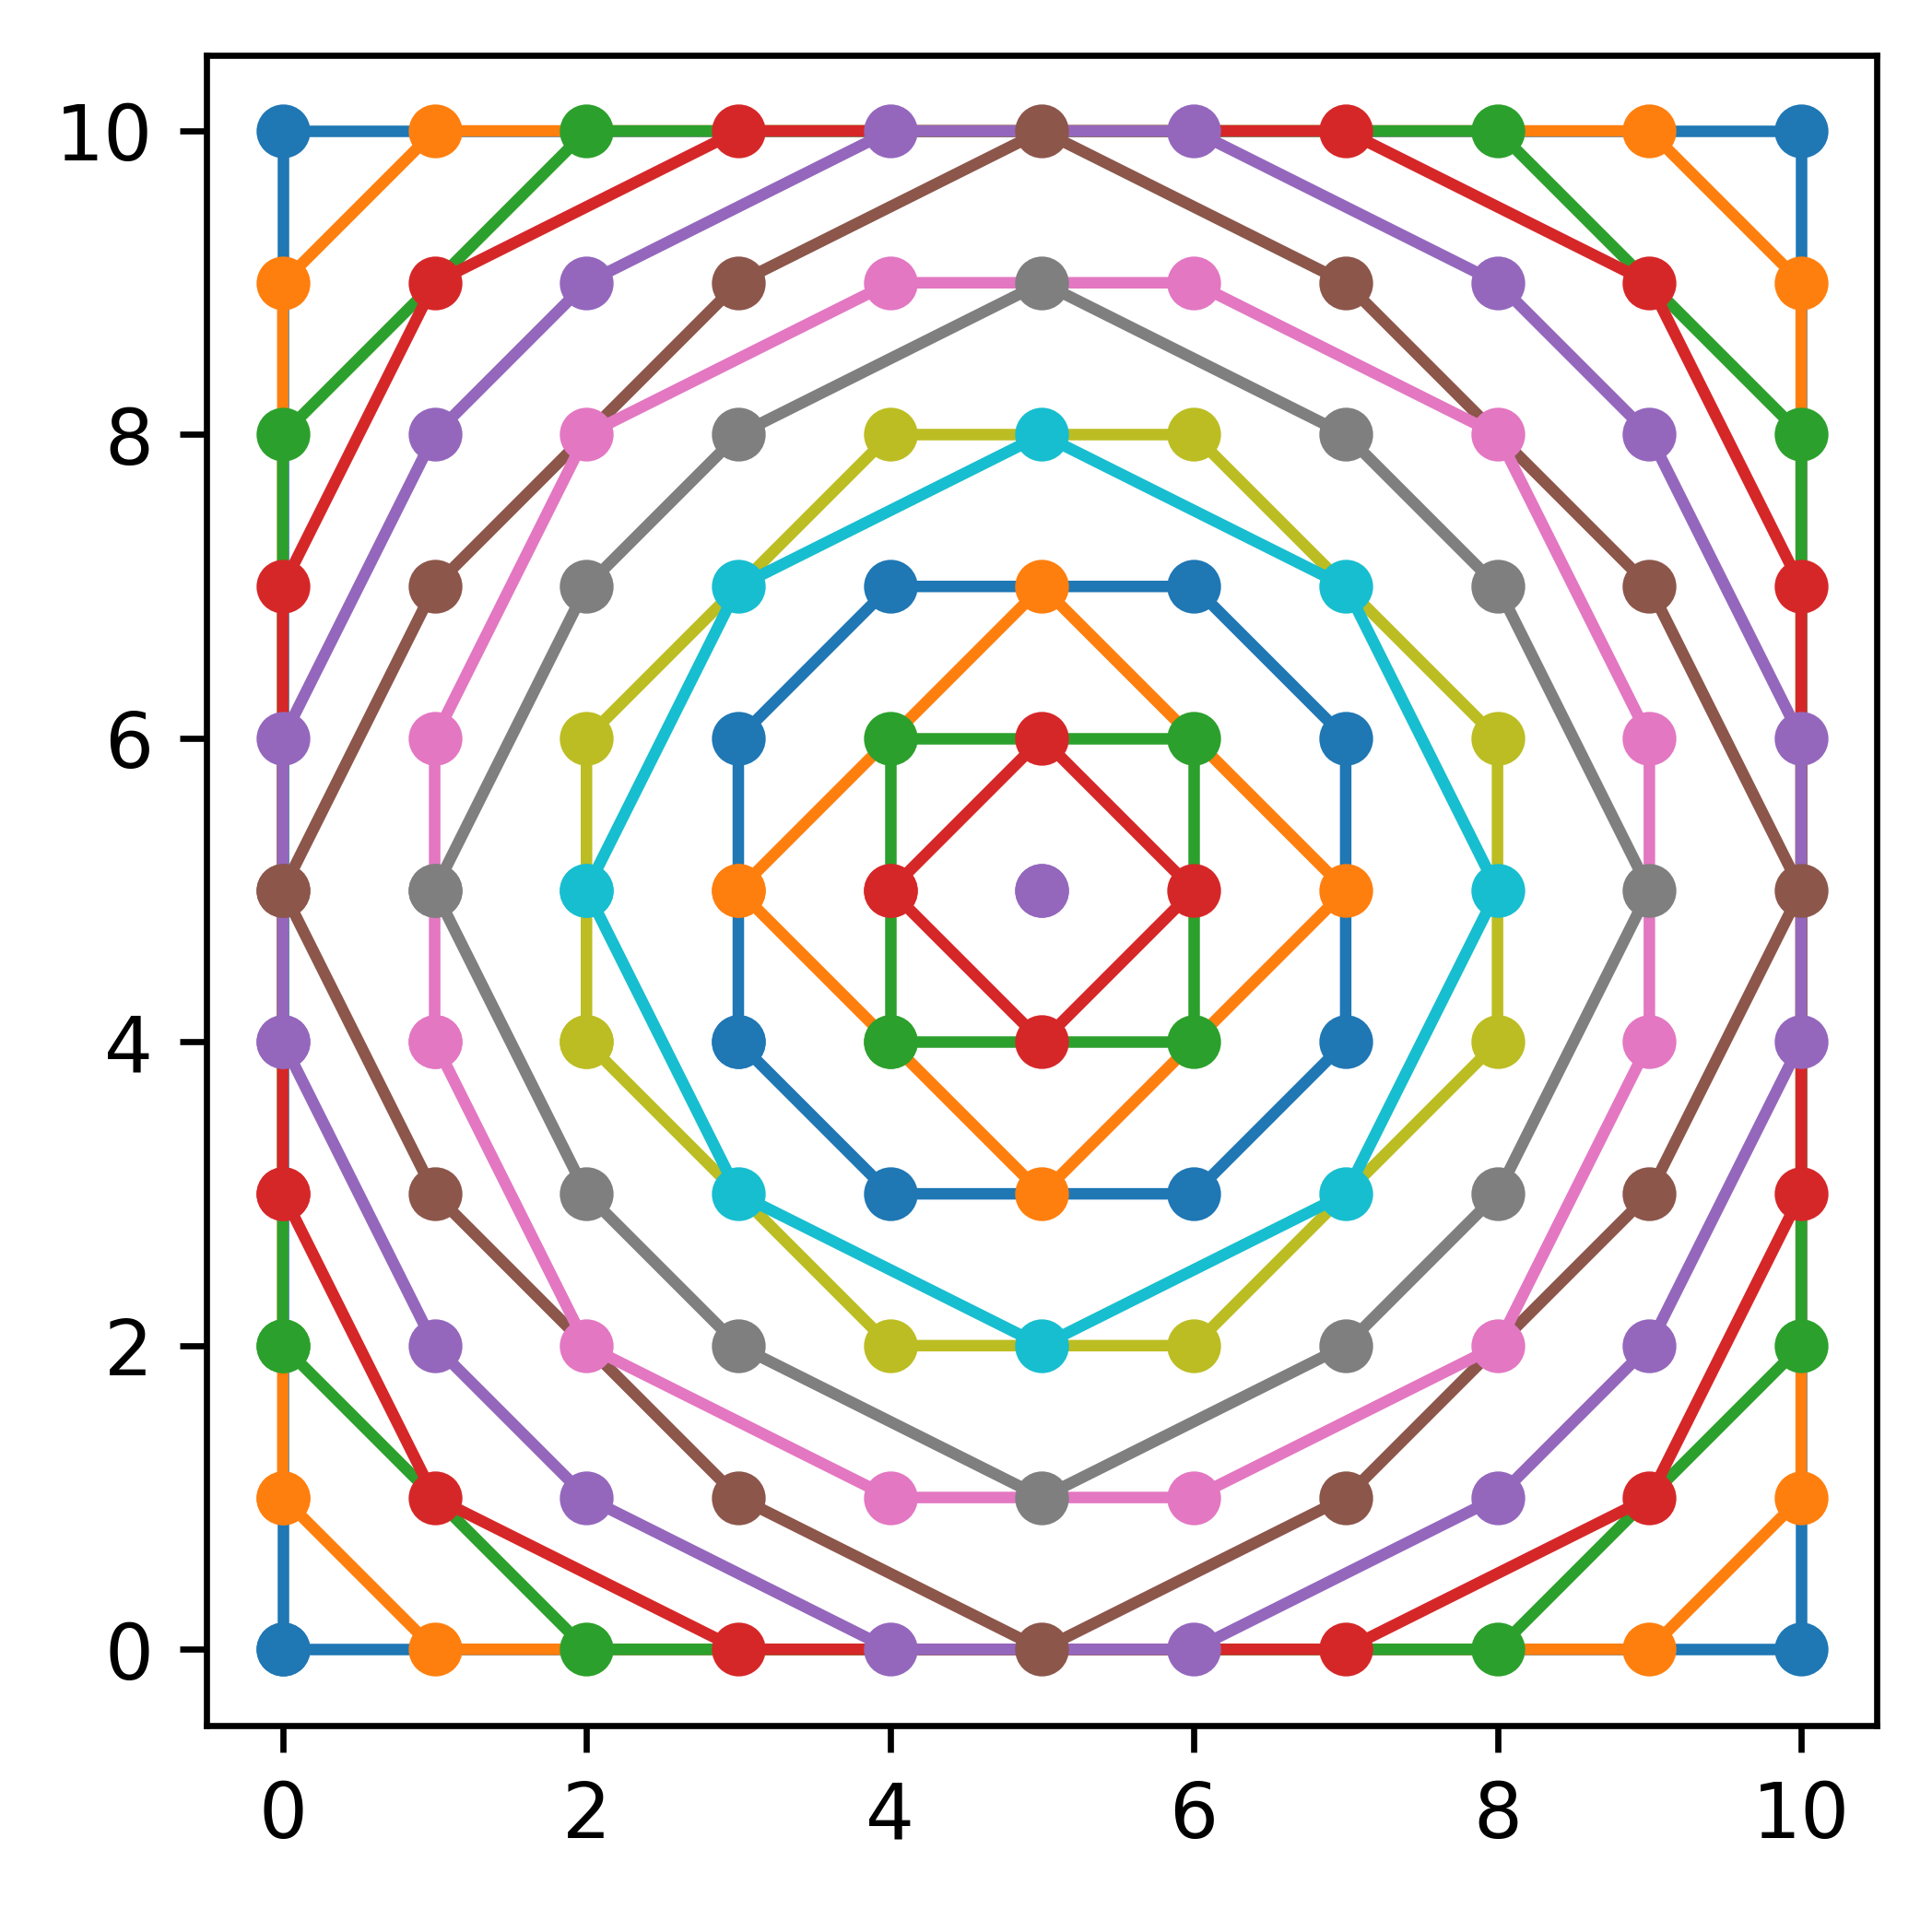
\includegraphics[scale=0.7]{11x11_enakomerna.png}
\end{figure}

\begin{figure}[h]
	\centering
	\caption{Postopek lupljenja ovojnic potenčne $5 \times 5$ mreže}
	\label{fig:5x5}
	\vspace{2mm}
	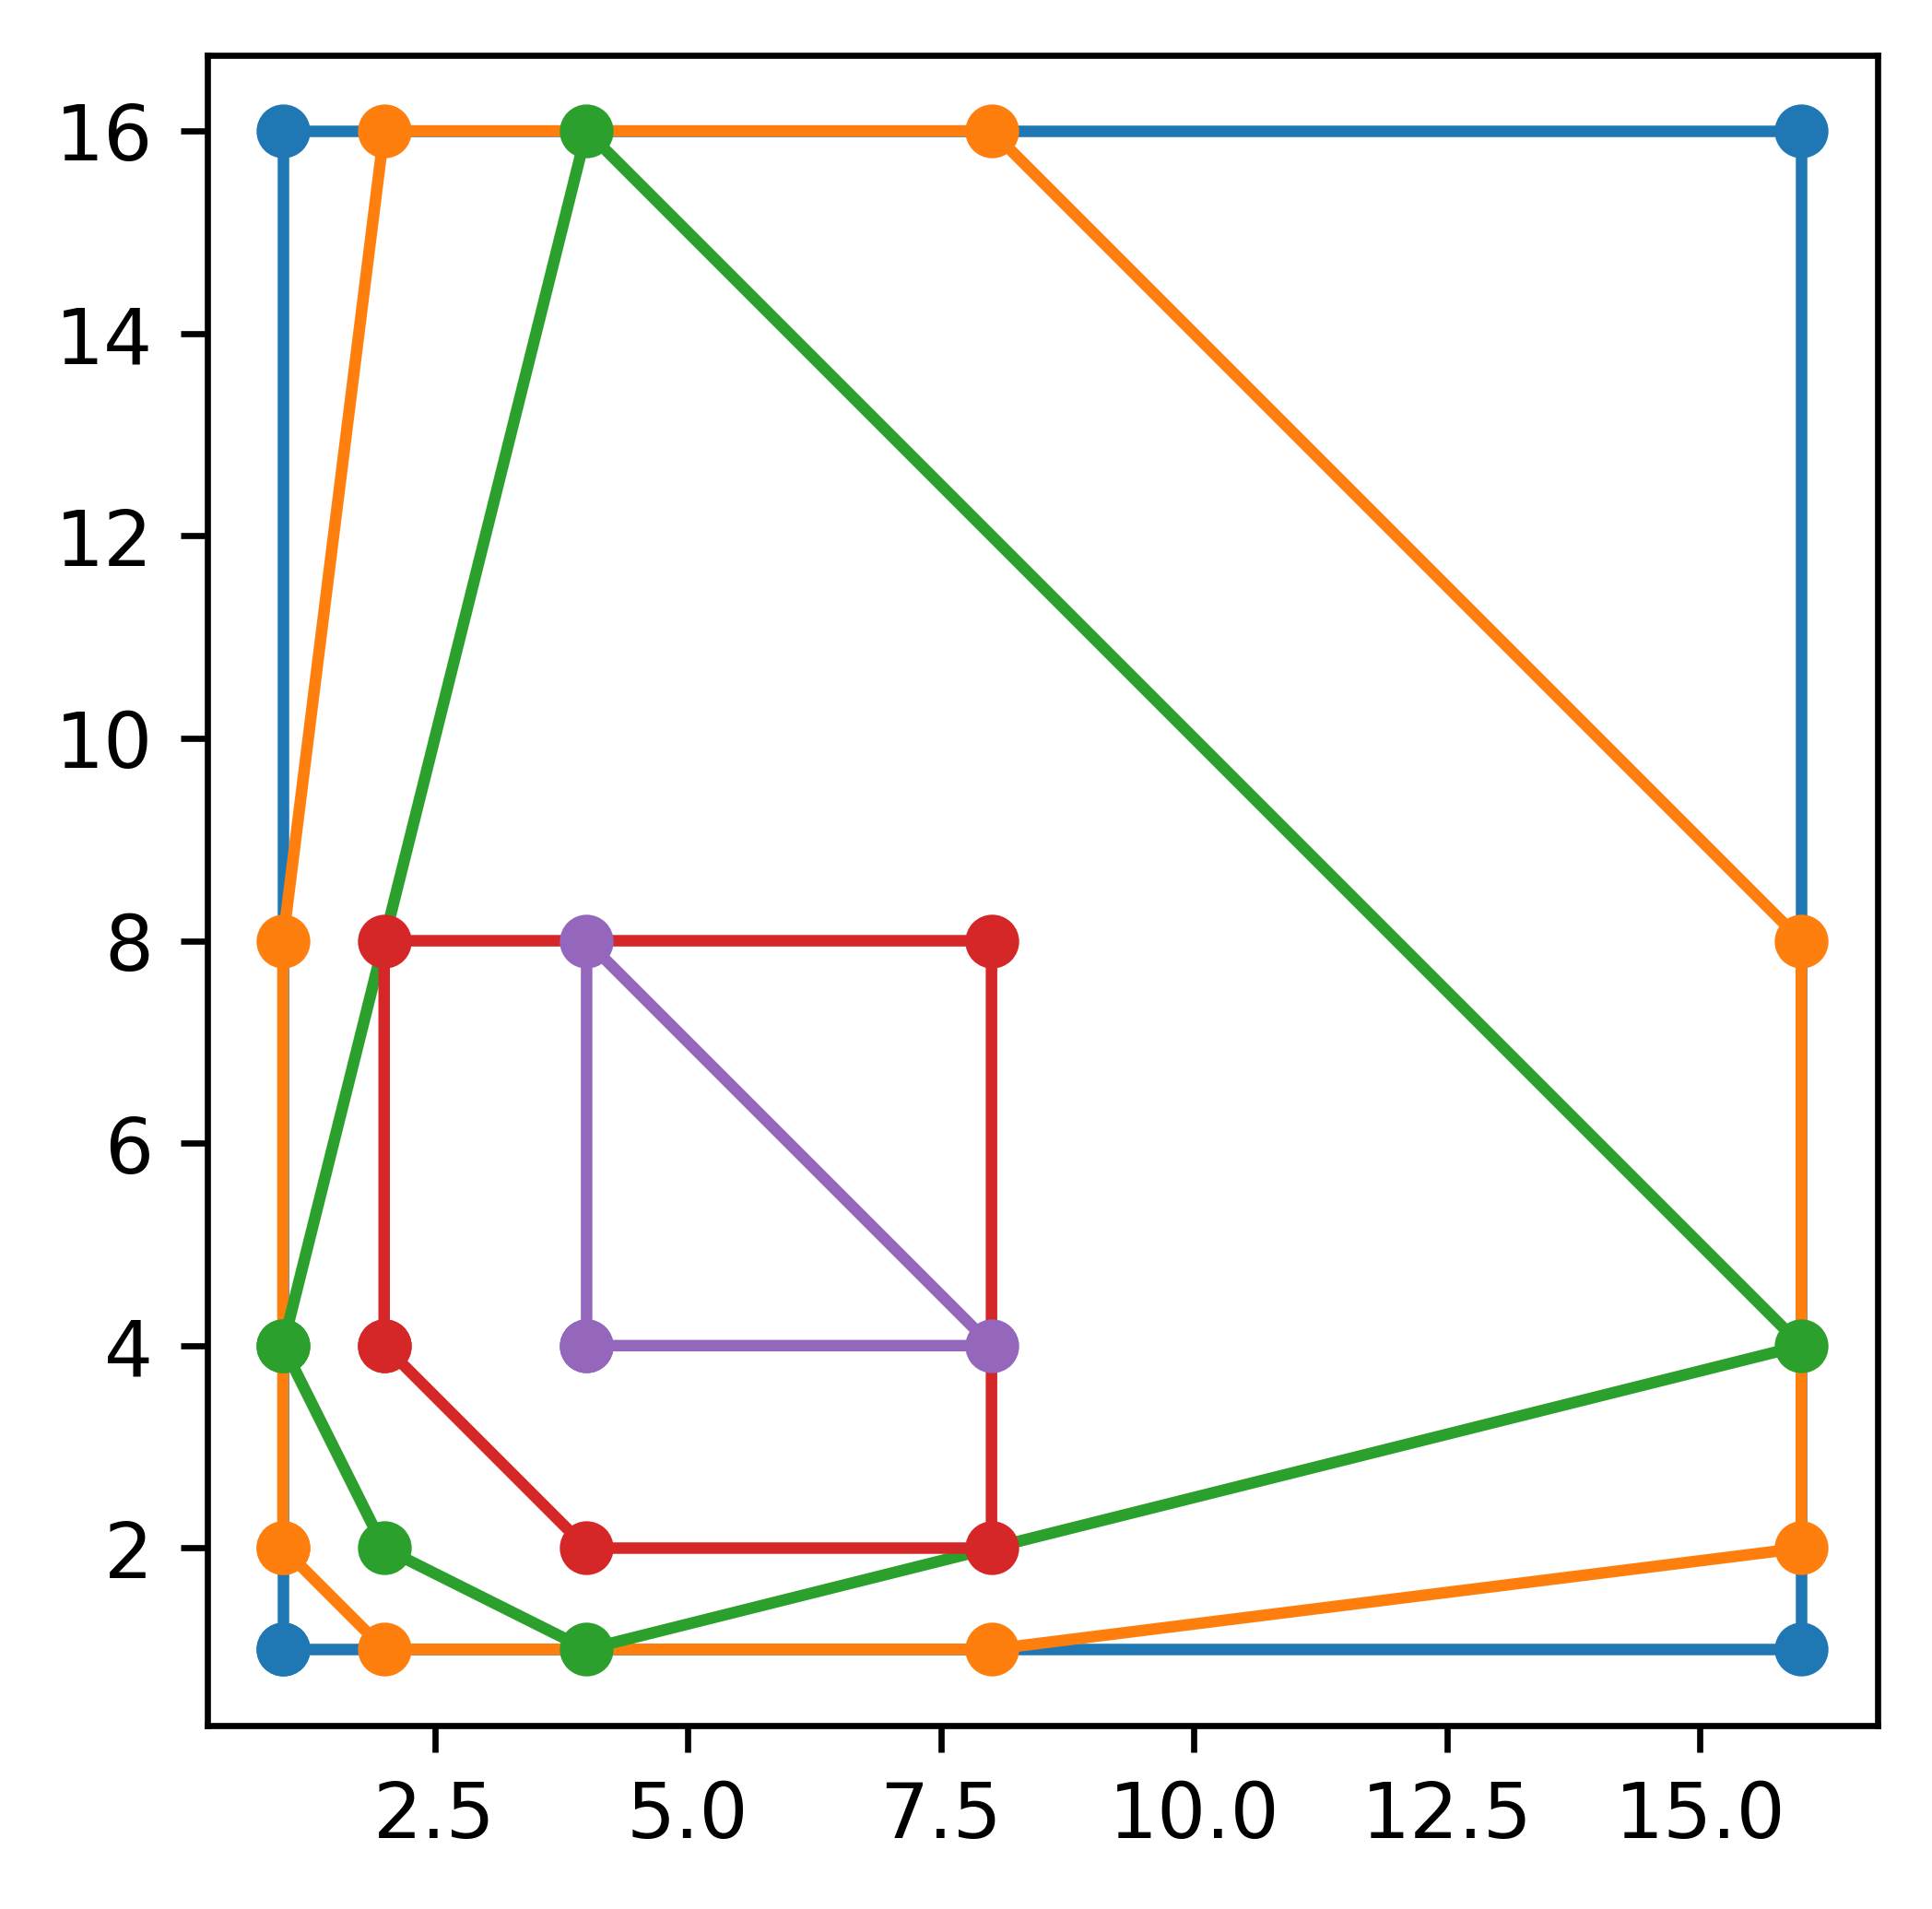
\includegraphics[scale=0.7]{5x5_potencna.png}
\end{figure}

\subsection{Časovna zahtevnost algoritma}

\begin{figure}[h]
	\centering
	\caption{Število ovojnic glede na $n$}
	\label{fig:st_ovojnic}
	\vspace{2mm}
	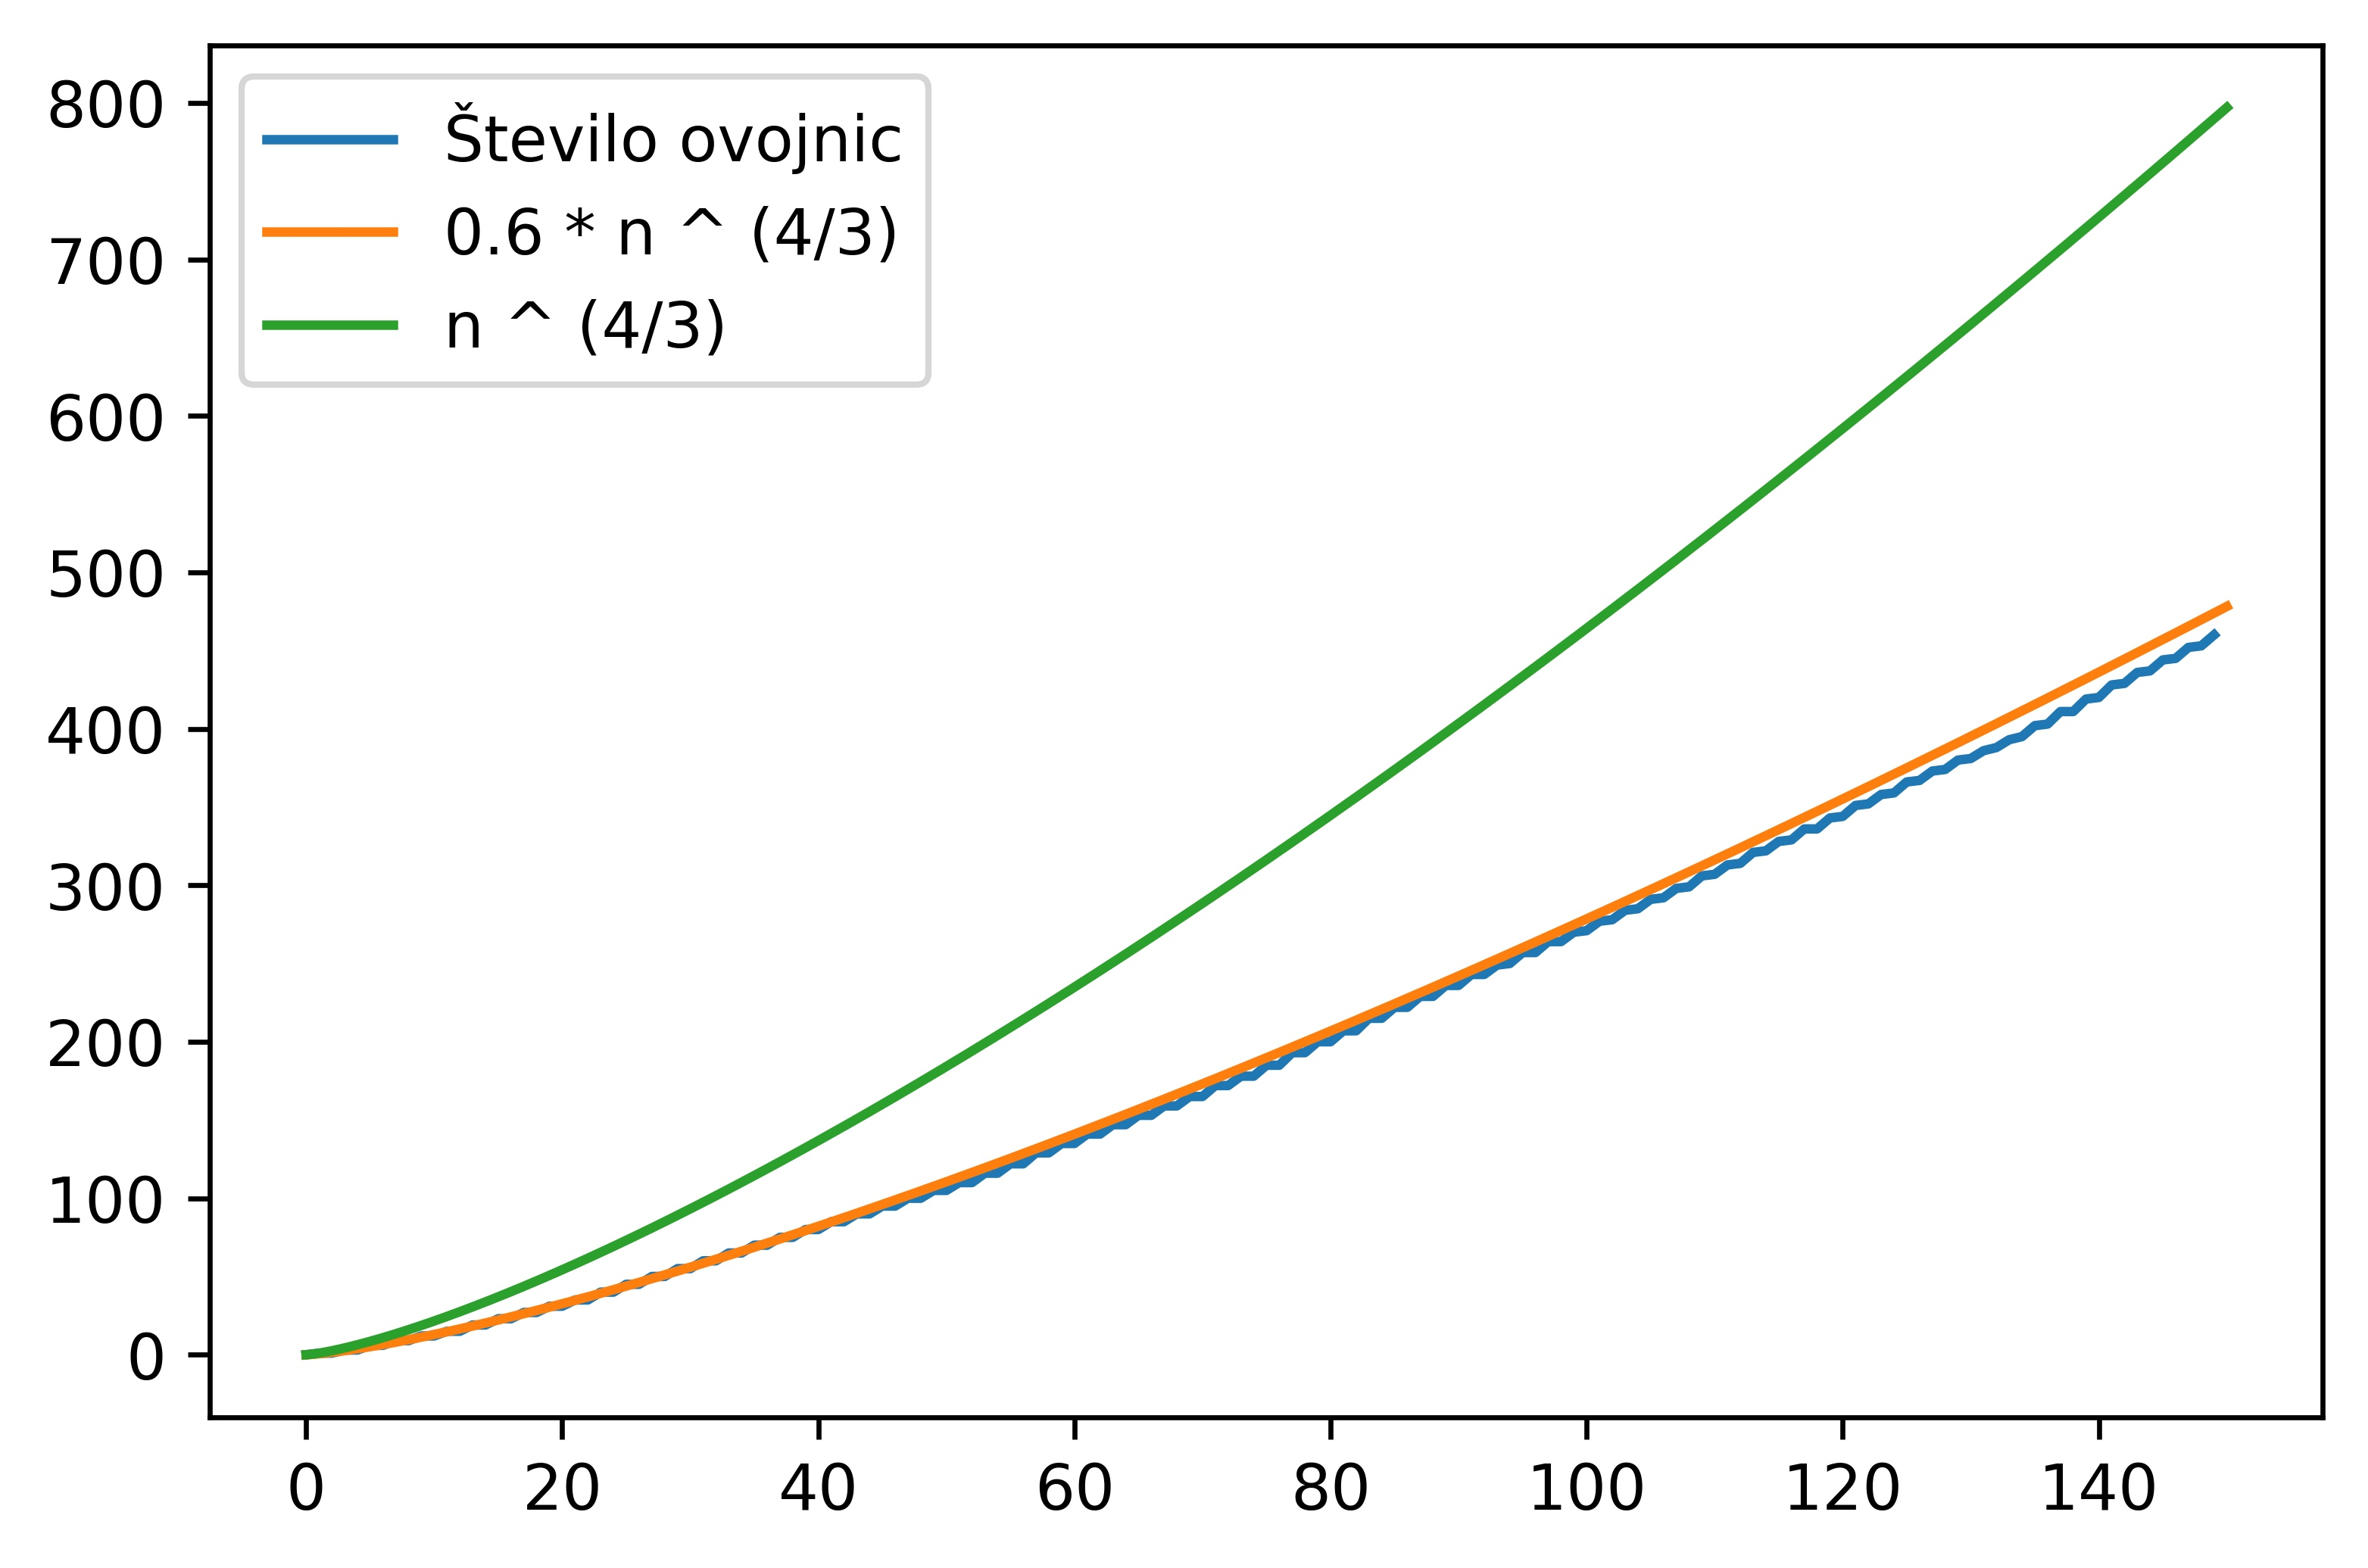
\includegraphics[scale=0.7]{st_ovojnic.jpg}
\end{figure}

\section{Rezultati}

\section{Zaključek}


\end{document}